%%%%%%%%%%%%%%%%%%%%%%%%%%%%%%%%%%%%%%%%%
% Masters/Doctoral Thesis 
% LaTeX Template
% Version 2.5 (27/8/17)
%
% This template was downloaded from:
% http://www.LaTeXTemplates.com
%
% Version 2.x major modifications by:
% Vel (vel@latextemplates.com)
%
% This template is based on a template by:
% Steve Gunn (http://users.ecs.soton.ac.uk/srg/softwaretools/document/templates/)
% Sunil Patel (http://www.sunilpatel.co.uk/thesis-template/)
%
% Template license:
% CC BY-NC-SA 3.0 (http://creativecommons.org/licenses/by-nc-sa/3.0/)
%
%%%%%%%%%%%%%%%%%%%%%%%%%%%%%%%%%%%%%%%%%

%----------------------------------------------------------------------------------------
%	PACKAGES AND OTHER DOCUMENT CONFIGURATIONS
%----------------------------------------------------------------------------------------

\documentclass[
11pt, % The default document font size, options: 10pt, 11pt, 12pt
oneside, % Two side (alternating margins) for binding by default, uncomment to switch to one side
english, % ngerman for German
singlespacing, % Single line spacing, alternatives: onehalfspacing or doublespacing
%draft, % Uncomment to enable draft mode (no pictures, no links, overfull hboxes indicated)
% nolistspacing, % If the document is onehalfspacing or doublespacing, uncomment this to set spacing in lists to single
%liststotoc, % Uncomment to add the list of figures/tables/etc to the table of contents
%toctotoc, % Uncomment to add the main table of contents to the table of contents
%parskip, % Uncomment to add space between paragraphs
%nohyperref, % Uncomment to not load the hyperref package
headsepline, % Uncomment to get a line under the header
%chapterinoneline, % Uncomment to place the chapter title next to the number on one line
% consistentlayout, % Uncomment to change the layout of the declaration, abstract and acknowledgements pages to match the default layout
]{MastersDoctoralThesis} % The class file specifying the document structure

\usepackage[utf8]{inputenc} % Required for inputting international characters
\usepackage[T1]{fontenc} % Output font encoding for international characters

\usepackage{mathpazo} % Use the Palatino font by default

\usepackage[backend=bibtex,style=authoryear,natbib=true]{biblatex} % Use the bibtex backend with the authoryear citation style (which resembles APA)

\addbibresource{../bibtex.bib} % The filename of the bibliography

\usepackage[autostyle=true]{csquotes} % Required to generate language-dependent quotes in the bibliography

%----------------------------------------------------------------------------------------
%	MARGIN SETTINGS
%----------------------------------------------------------------------------------------

\geometry{
	paper=a4paper, % Change to letterpaper for US letter
	inner=2.5cm, % Inner margin
	outer=3.8cm, % Outer margin
	bindingoffset=.5cm, % Binding offset
	top=1.5cm, % Top margin
	bottom=1.5cm, % Bottom margin
	%showframe, % Uncomment to show how the type block is set on the page
}

%----------------------------------------------------------------------------------------
%	THESIS INFORMATION
%----------------------------------------------------------------------------------------

\thesistitle{SoPa++: Leveraging explainability from hybridized RNN, CNN and weighted finite-state neural architectures} % Your thesis title, this is used in the title and abstract, print it elsewhere with \ttitle
\supervisor{Dr. Sharid \textsc{Loáiciga} \\ University of Potsdam} % Your supervisor's name, this is used in the title page, print it elsewhere with \supname
\examiner{Mathias \textsc{Müller} \\ University of Zurich} % Your examiner's name, this is not currently used anywhere in the template, print it elsewhere with \examname
\degree{Cognitive Systems: Language, \\Learning, and Reasoning (M.Sc.)} % Your degree name, this is used in the title page and abstract, print it elsewhere with \degreename
\author{Atreya \textsc{Shankar}} % Your name, this is used in the title page and abstract, print it elsewhere with \authorname
\addresses{} % Your address, this is not currently used anywhere in the template, print it elsewhere with \addressname

\subject{Computational Linguistics} % Your subject area, this is not currently used anywhere in the template, print it elsewhere with \subjectname
\keywords{} % Keywords for your thesis, this is not currently used anywhere in the template, print it elsewhere with \keywordnames
\university{\href{https://www.uni-potsdam.de/en/university-of-potsdam}{University of Potsdam}} % Your university's name and URL, this is used in the title page and abstract, print it elsewhere with \univname
\department{\href{https://www.uni-potsdam.de/en/ling/index}{Department of Linguistics}} % Your department's name and URL, this is used in the title page and abstract, print it elsewhere with \deptname
\group{\href{http://clp.ling.uni-potsdam.de/}{Foundations of Computational Linguistics Research Group
}} % Your research group's name and URL, this is used in the title page, print it elsewhere with \groupname

\AtBeginDocument{
\hypersetup{pdftitle=\ttitle} % Set the PDF's title to your title
\hypersetup{pdfauthor=\authorname} % Set the PDF's author to your name
\hypersetup{pdfkeywords=\keywordnames} % Set the PDF's keywords to your keywords
}


\begin{document}

\frontmatter % Use roman page numbering style (i, ii, iii, iv...) for the pre-content pages

\pagestyle{plain} % Default to the plain heading style until the thesis style is called for the body content

%----------------------------------------------------------------------------------------
%	TITLE PAGE
%----------------------------------------------------------------------------------------

\begin{titlepage}
\begin{center}

\vspace*{.06\textheight}
{\scshape\LARGE \univname\par}\vspace{1.5cm} % University name
\textsc{\Large Master's Thesis}\\[0.5cm] % Thesis type

\HRule \\[0.4cm] % Horizontal line
{\huge \bfseries \ttitle\par}\vspace{0.4cm} % Thesis title
\HRule \\[1.5cm] % Horizontal line
 
\begin{minipage}[t]{0.4\textwidth}
\begin{flushleft} \large
\emph{Author:}\\
\href{https://www.linkedin.com/in/atreya-shankar-644352113}{\authorname} % Author name - remove the \href bracket to remove the link
\end{flushleft}
\end{minipage}
\begin{minipage}[t]{0.4\textwidth}
\begin{flushright} \large
\emph{1st Supervisor:} \\
\href{https://sites.google.com/site/loaicigasharid/portada}{\supname} \\[5pt] % Supervisor name - remove the \href bracket to remove the link
\emph{2nd Supervisor:} \\
\href{https://www.uzh.ch/cmsssl/cl/de/people/team/compling/mmueller.html}{\examname} % Supervisor name - remove the \href bracket to remove the link  
\end{flushright}
\end{minipage}\\[3cm]
 
\vfill

\large \textit{A thesis submitted in fulfillment of the requirements\\ for the degree of \degreename}\\[0.3cm] % University requirement text
\textit{in the}\\[0.4cm]
\groupname\\\deptname\\[2cm] % Research group name and department name
 
\vfill

{\large \today}\\[4cm] % Date
%\includegraphics{Logo} % University/department logo - uncomment to place it
 
\vfill
\end{center}
\end{titlepage}

%----------------------------------------------------------------------------------------
%	LIST OF CONTENTS/FIGURES/TABLES PAGES
%----------------------------------------------------------------------------------------

\tableofcontents % Prints the main table of contents

%----------------------------------------------------------------------------------------
%	THESIS CONTENT - CHAPTERS
%----------------------------------------------------------------------------------------

\mainmatter % Begin numeric (1,2,3...) page numbering

\pagestyle{thesis} % Return the page headers back to the "thesis" style

% Include the chapters of the thesis as separate files from the Chapters folder
% Uncomment the lines as you write the chapters

\chapter{Introduction}

\label{chapter:introduction}

In this chapter, we introduce this thesis by presenting its motivation,
describing our research questions and providing an overview of the thesis
structure.

\section{Motivation and objective}

There is a recent trend of increasingly complex deep learning models achieving
state-of-the-art performance on \ac{ml} and \ac{nlp} tasks, as shown in Figure
\ref{fig:nlp_progress}. To address emerging concerns such as security risks and
inductive biases, several studies argue for focused research into \ac{xai}
\citep{doran2017does,townsend2019extracting,danilevsky2020survey,arrieta2020explainable}.
Of these studies, \citet{arrieta2020explainable} provide an extensive overview
of \ac{xai} and related concepts based on a thorough literature review of
$\sim$400 \ac{xai} research contributions published to date. In particular,
\citet{arrieta2020explainable} explore and classify a variety of \ac{ml} models
into transparent and black-box categories depending on their degrees of
transparency. Furthermore, they explore taxonomies of post-hoc explainability
techniques aimed at effectively explaining black-box models. Notable
explainability techniques used in recent research include local explanations,
feature relevance and explanations by simplification.

Through our own survey of recent literature on explainability techniques in
\ac{nlp}, we came across several interesting studies employing the three
aforementioned post-hoc explainability techniques to better explain deep neural networks
\citep{schwartz2018sopa,peng2018rational,suresh-etal-2019-distilling,wang2019state,jiang2020cold}.
Of these studies, we draw inspiration from \citet{schwartz2018sopa} who
developed the novel hybridized \ac{rnn}, \ac{cnn} and weighted finite-state
\ac{sopa} model architecture with a special focus in model explainability. While
the \ac{sopa} model functions well, we find its explainability techniques to be
localized and indirect despite its neural architecture being suited for the
globalized and direct explanations by simplification explainability technique.
The main objective of this thesis is to address these limitations and to propose
a modified model, \textbf{\ac{spp}}, which could allow for effective explanations
by simplification. To facilitate this objective, we study both the performance and
explanations by simplification of the modified \ac{spp} model on the recently
released \ac{fmtod} data set from \citet{schuster-etal-2019-cross-lingual};
focusing on the English-language intent classification task.

\begin{figure}[t!]
  \centering
  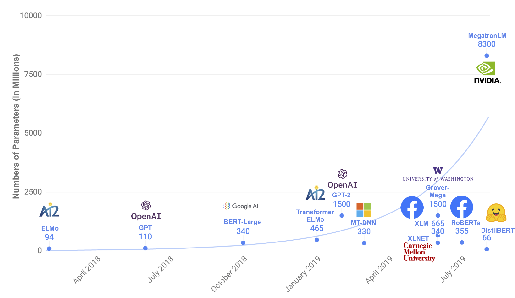
\includegraphics[width=13cm]{pdfs/borrowed/nlp_sota_model_size_progress.pdf}
  \caption{Parameter counts of recently released pre-trained language models
    which showed competitive or state-of-the-art performance when fine-tuned
    over a range of NLP tasks; figure taken from \citet{sanh2019distilbert}}
  \label{fig:nlp_progress}
\end{figure}

\section{Research questions}

\label{section:rq}

To guide us in addressing our objective, we aim to answer the following three
research questions:

\begin{enumerate}
  \item Does \ac{spp} provide competitive\footnote{We define
    competitive performance as the scenario where a mean performance metric on a
    certain task falls within the range obtained from other recent studies on
    the same task} performance on the \ac{fmtod} English language intent classification task?
  \item To what extent does \ac{spp} contribute to effective explanations by
  simplification on the \ac{fmtod} English language intent classification task?
  \item What interesting and relevant explanations can \ac{spp} provide on the
  \ac{fmtod} English language intent classification task?
\end{enumerate}

\section{Thesis structure}

We now summarize the contents and structure of this thesis.

\begin{description}[align=left]
  \item [Chapter \ref{chapter:introduction}:] Introduce this thesis, its
  contents and our research questions.
  \item [Chapter \ref{chapter:background}:] Describe the background concepts
  utilized in this thesis.
  \item [Chapter \ref{chapter:methodologies}:] Describe the \ac{fmtod} data set and
  methodologies pursued in this thesis.
  \item [Chapter \ref{chapter:results}:] Describe the results obtained from our
  methodologies.
  \item [Chapter \ref{chapter:discussion}:] Interpret the results and discuss their
  implications.
  \item [Chapter \ref{chapter:conclusions}:] Summarize the findings
  of this thesis.
  \item [Chapter \ref{chapter:further_work}:] Describe future work to expand on
  our research questions.
\end{description}

% LocalWords:  explainability pre NLP

%%% Local Variables: 
%%% mode: latex
%%% TeX-master: "main"
%%% End:

%----------------------------------------------------------------------------------------
%	BIBLIOGRAPHY
%----------------------------------------------------------------------------------------

\nocite{*}
\printbibliography[heading=bibintoc]

%----------------------------------------------------------------------------------------

\end{document}  